\subsection{Hagen-Poiseuille Flow}

In the previous test case the channel walls were aligned parallel to the simulation grid. Hence, no further interpolation procedures
are necessary to mimic the exact boundaries.
In order to test the accuracy of the VF and the IP method a test case with a curved geometry is necessary.
Furthermore it is possible to investigate the discretization error of the non-interpolating VP and DF method, with respect to curved geometries.

A simple adaption of the planar Poiseuille flow, is the laminar flow through a pipe, also referred to as Hagen-Poiseuille flow \citep{tritton88}.
The setup of the fluid domain is schematically shown in Fig. \ref{validation:setup_hpflow}.
It consist of a circular pipe with the radius $r_0$, which extends infinitely parallel to the $x$ axis.
This is similar to Sec. \ref{vali:sec_lpflow_setup} realized by using periodic boundaries in $x$-direction
and immersed boundaries for the channel wall.
The center of the pipe is set to the center of the simulation domain ${(y_0, z_0) = (\nicefrac{l_y}{2}, \nicefrac{l_z}{2})}$.
In analogy to the Poiseuille flow, the velocity profile is a result from a predfined pressure gradient $\nicefrac{\partial p}{\partial x}$ in x-direction,
which  is added into the Navier-Stokes equation as an additional forcing term.

\begin{figure}[!bp]
      \centering
        \resizebox{0.75 \textwidth}{!}{
       \import{gfx/immersed_boundary/hpflow///}{setup.pdf_tex}
      }
      \caption{Setup for the Hagen-Poiseuille flow, given be a pipe of radius $r_0$ with the center at  ${(\nicefrac{l_y}{2}, \nicefrac{l_z}{2})}$ and of infinitesimal length.}
\end{figure}

For an analytical solution of this problem we refer to \citep{Kundu2012}.
Once again a steady state flow can be assumed, which implies that $\partial v_x/\partial t = 0$. With the introduction of cylindrical coordinates $(r, \phi, x)$
and the assumption that the flow is independent of $\phi$ the equation of motion reduces to

\begin{align}
    \label{vali:hpflow:navstok}
        0 &= - \frac{\partial p}{\partial x}  +  \frac{1}{\Rey} \frac{1}{r}\frac{\partial}{\partial r}\left(r\frac{\partial v_x}{\partial r}\right)
\end{align}

where $Re = \nicefrac{V_{m}r_0}{\nu}$.
The non-dimensional scales are similar to Sec. \ref{vali:sec_lpflow_setup}  except that the length scale is set to $r_0$ instead of $\Delta h$.

The integration of Eq. \ref{vali:hpflow:navstok} gives
\begin{align}
    v_x(r) &= \frac{r^2}{4}\frac{\partial p}{\partial x}\Rey + A \ln r + B
\end{align}

It holds that $v_x(0)= V_{\text{M}}$ this condition can only be fullfilled if $A=0$.
With the use of the boundary conditions $u(r_0) = 0$ the velocity profile is given by
\begin{align}
    v_x(r) &= \frac{r^2 - r_0^2}{4}\frac{\partial p}{\partial x}Re
\end{align}
Since $V_{M} \stackrel{!}{=} 1$ by definition, the pressure condition for the domain needs to be set to
\begin{align}
    \frac{\partial p}{\partial x} = -\frac{4 r_o^2}{Re}
\end{align}

\subsection{Simulations}

\subsubsection{Grid Convergence Study with comparsion to the Theoretical Solution}

For an error evaluation a grid convergence study was performed with the Reynolds number set to $Re=100$.
The number of grid points was varied in the intervall $N\in[32, 256]$ furthermore a
simulation with a resolution of $N=512$ was carried out.
Since the maximum velocity of the channel is given by $V_{M}=1$, due to the choice of non-dimensionalization,
the sound speed was set to $c^2 = 100$ to fullfill the incompressibilty condition $Ma = v/c < 0.1$.
The resulting timestep for the highest resolution is $\Delta t = 1e-4$.
The main parameters of the simulation are  given by

\begin{center}
\vspace*{0.7ex}
\begin{tabular}{c|c|c|c|c|c|c|c }
 $ N  $                   & $\Delta t$ & $\Delta z$            & $\Rey$  & $c^2$   & $l_y, l_z$ & $r_0$ & $T_{end}$\\
\hline
 $512, [16, 256], \Delta N = 16 $& $10^{-4}$ & $\nicefrac{1}{N}$ & 500     & $500$   & (2.5, 2.5) & 1     & 20\\
\end{tabular}
\vspace*{0.7ex}
\end{center}

With this setup the VP, DF and IP method were tested with FD2 and FD4 methods and optional with the VF method.
The IP method was additionally tested with the DF method. Thus, the velocity is interpolated on the
immersed boundary and set to zero outside of fluid domain.
For the VP method the non-dimensionalized damping was set to $J=10^{-4}$.
It would be possible to choose a larger time step for the lower resolution cases, which means that in general
one would apply a larger $J$ in a case of an applicaton, due to the stability criterion $J>\Delta t$.
As a results the damping force on the boundaries $\propto \nicefrac{1}{J}$ would be smaller.
To remain consistent in the error convergence, here $\Delta t$ and
therefore $J$ are not altered.

\subsubsection{Long-Term Simulations}

In Order to test the  numerical stability and conservation of mass, a long-term simulation was performed.
A Reynolds number of $Re=100$ was chosen. The resolution is set to $N=96$ grid points and
the ending time was set to $T_{\text{end}}=1600$.
The main parameters of the simulation are  given by

\begin{center}
\vspace*{0.7ex}
\begin{tabular}{c|c|c|c|c|c|c|c }
 $ N  $                   & $\Delta t$ & $\Delta x$            & $\Rey$  & $c^2$   & $l_y, l_z$ &$r_0$ & $T_{end}$\\
\hline
 $96 $& $10^{-4}$ & $\nicefrac{1}{N}$ & 500     & $500$   & (2.5, 2.5)  & 1     & 10\\
\end{tabular}
\vspace*{0.7ex}
\end{center}

With this setup the same methods as in the grid convergence study were tested.

\subsection{Results}

\subsubsection{Grid Convergence Study}

The results of the grid convergence study are shown from Fig. \ref{vali:hp_flow_gc_vp} to Fig. \ref{vali:hp_flow_gc_all}.
For a better overview the results are distributed into four plots.
For all methods (except IP+DF-FD4) an approximately linear decrease in the double logarithmic space can be observed.

In Fig. \ref{vali:hp_flow_gc_vp} the relative $l_2$-error is shown for different VP-methods.
For the default VP-method with FD2 and FD4 the error converges rate is about $\lambda=1.17$,
the FD4 has a slightly smaller error than the FD2 method..
The optional use of the VF-method improves the error converges to about $\lambda=1.65$,
here the FD2 method has a slightly smaller error.
It can be noted that the overall error is smaller ($\approx 10^{-2}$ for $N=100$)
when using the VP-VF-method in comparison to the VP-method ($\approx2\cdot 10^{-2}$ for $N=100$)

In Fig. \ref{vali:hp_flow_gc_df} the relative $l_2$-error is shown for different DF-methods.
For the default DF-method with FD2 and FD4 the error convergence rate is about $\lambda=1.2$,
again FD4 has a smaller error than FD2.
The optional use of the VF-method improves the error convergence to about $\lambda=1.4$,
which is worse in comparison to the VP-method. The FD2 method has a smaller error then FD4 method when using VF.
The overall error is smaller ($\approx 1.5 \cdot 10^{-2}$ for $N=100$) for the DF-VF-method,
in comparsion to the DF-method ($\approx2\cdot 10^{-2}$ for $N=100$)

In Fig. \ref{vali:hp_flow_gc_ip} the relative $l_2$-error is shown for different IP-methods.
For the IP-FD4 method the decay rate is about $1.4$.
For the IP-FD2 and IP+DF-FD2 method the errors are identical, the decay rate is about $2.4$
The IP+DF-FD4 method is numerically not stable and therefore not shown.
From the interpolation methods the IP-o2 method gives the smallest error  ($\approx 5 \cdot 10^{-5}$ for $N=100$).

Finally Fig. \ref{vali:hp_flow_gc_all} shows the methods  with the best convergence
rates from the different DF, VP and IP methods in one plot.
In summary it can be said that the overall convergence rate of the IP-FD2-method is of one order better
than the VP-VF and DF-VF methods. The relative error of the interpolation method ranges
between one and two order of magnitudes below all other methods, depending on the resolution.

\begin{figure}[!bp]
  \begin{minipage}[c]{0.5\textwidth}
      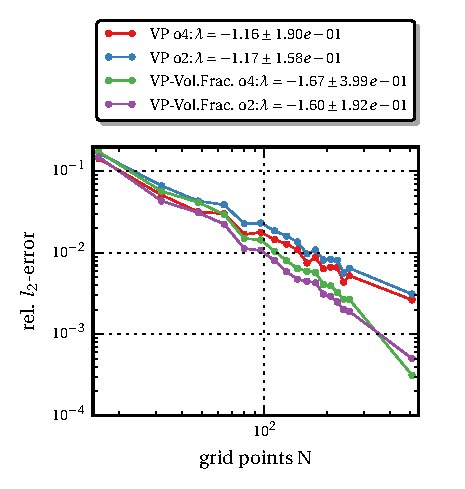
\includegraphics{gfx/immersed_boundary/hpflow/theo/vp.pdf}
      \caption{\label{vali:hp_flow_gc_vp}
          Relative $l_2$-error for different Volume-Penalization methods.}
  \end{minipage}
  \begin{minipage}[c]{0.5\textwidth}
      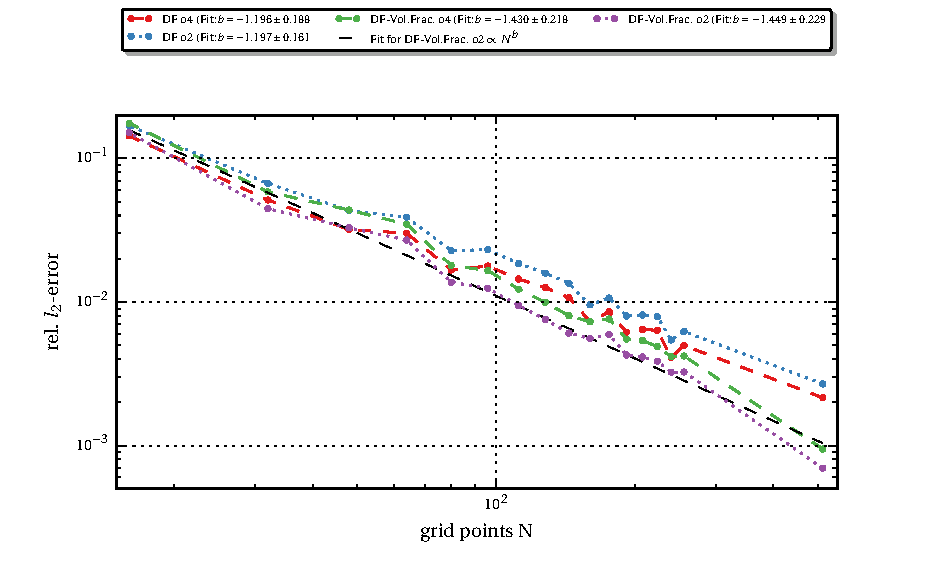
\includegraphics{gfx/immersed_boundary/hpflow/theo/df.pdf}
      \caption{\label{vali:hp_flow_gc_df}
          Relative $l_2$-error for different Direct-Forcing methods.}
  \end{minipage}
  \begin{minipage}[c]{0.5\textwidth}
      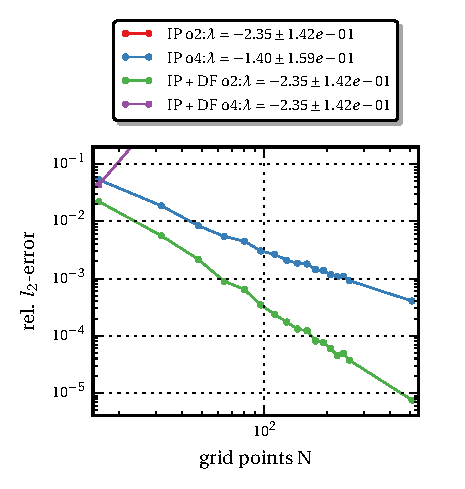
\includegraphics{gfx/immersed_boundary/hpflow/theo/ip.pdf}
      \caption{\label{vali:hp_flow_gc_ip}
          Relative $l_2$-error for different Interpolation methods.}
  \end{minipage}
  \begin{minipage}[c]{0.5\textwidth}
      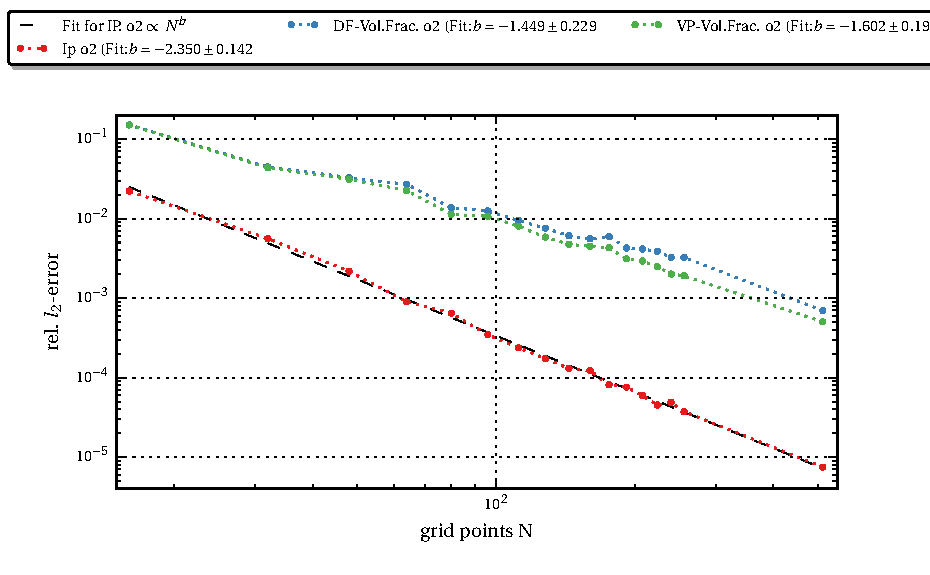
\includegraphics{gfx/immersed_boundary/hpflow/theo/all.pdf}
      \caption{\label{vali:hp_flow_gc_all}
          Relative $l_2$-error for the methods with the smallest error in comparsion.}
  \end{minipage}
\end{figure}

\subsubsection{Long-Term Simulations}

The long-term simulations were performed in order to test the numerical-stability and the conservation of mass.
For all methods, except the IP-DF4 method, these simulation were numerically stable.
The density was averaged of the fluid domain by

\begin{align}
    \left<\rho(t)\right> \frac{\int_V \dif V \rho(x,y,z)}{\int_V \dif V} =
    \frac{1}{N}\left(\sum_{i,j,k}^{N_x, N_y, N_z} \rho_{i,j,k}\right)
\end{align}


For all FD2 methods the averaged density is zero, which indicates that the total mass flux through the
fluid domain boundaries is zero.
It can be seen that for all FD4 methods oscillations in the density emerge.
This is exemplariliy shown in Fig.  \ref{hpflow:results_long_ts} for the DF-VF-FD4 method.
The profile of the other DF4 methods of is shown in Appendix \ref{fig:hpflow_allgc_theo}.

Finally in Fig. \ref{hpflow:results_long_example} the averaged density with respect to the simulation time is, shown for the
FD4 methods.  For the VP and DF methods the density increases to above $5\cdot10^{-5}$.
The VF methods have a decrease in the density, which is remains of the order $10^{-4}$.
For all FD4 methods the change in the averaged density is followed by a saturation.

\begin{figure}[!bp]
  \begin{minipage}[c]{0.5\textwidth}
      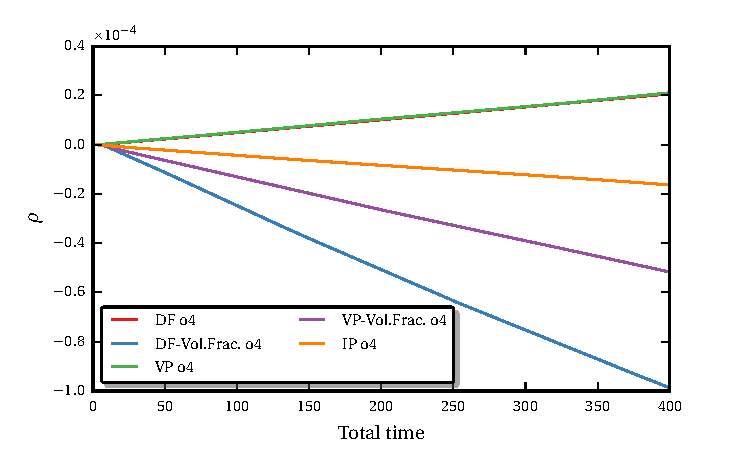
\includegraphics{gfx/immersed_boundary/hpflow/long/ts.pdf}
      \caption{\label{hpflow:results_long_ts}
            Averaged density for FD4 metdods with respect to the simulation time.
          }
  \end{minipage}
  \begin{minipage}[c]{0.5\textwidth}
      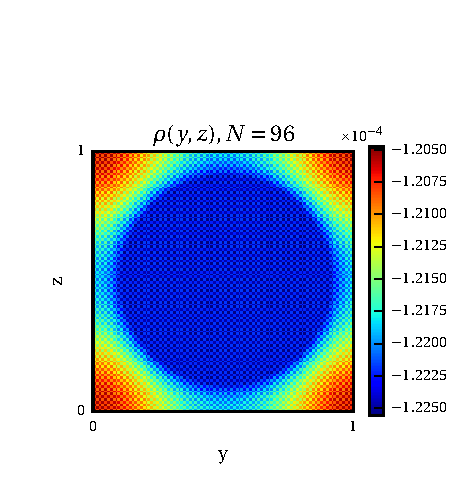
\includegraphics{gfx/immersed_boundary/hpflow/long/example.pdf}
      \caption{\label{hpflow:results_long_example}
        Density in the xy plane at $T_{\text{end}}=1600$, for the DF-VP-FD2 method.
      }
  \end{minipage}
\end{figure}

\clearpage

\subsection{Discussion}

-all method



-alle methoden except ip haben gleiche fehler ordnung
-fraction methdos is a little bit better
-ip ist am besten mit 2 ordnung

-the best error is interpolation

- ip o4 unstable mit mit DF o4 possible explanation is given in sec. .
- density reaches over the simulation domain


- warum ist ip unstable ???
- ip o2 identical to o4


 The identy of these methods occurs due to the decoupling of the velocity fields
on the border ot the fluid domain. Since the interpolation stencil seperates the fluid and wall domain, the 2nd order
stencil doesn't see any points in the wall domain, therefore there is no difference in using the direct forcing method.\\

\subsubsection{Long-Term Simulations}
- density changes
- interpolation at the boarders
- a part goes into immersed boundar
- howerver the overall influence can be neglected
- explanation decoupling of the pressure


